\section{Описание предметной области}
\subsection{Алгоритмическая покупка рекламы}
\subsubsection{Основные термины и понятия}

Алгоритмическая покупка рекламы --- это способ автоматизированной доставки цифровой рекламы (например, 
рекламного содержимого интернет страниц) в режиме реального времени, основанный на индивидуальных 
особенностях каждого отдельного события доставки.

\begin{figure}[h!]
    \centering
    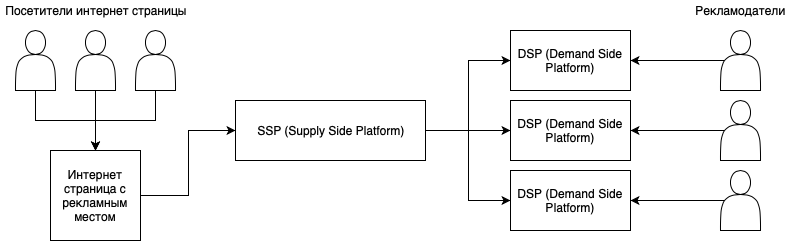
\includegraphics[width=0.9\textwidth]{inc/images/rtb.png}
    \caption{Схема алгоритмической покупки рекламы}
    \label{img:pragrammatic-advertising}
\end{figure}

На рисунке \ref{img:pragrammatic-advertising} отображена схема модели алгоритмической покупки рекламы
RTB (Real-Time Bidding, покупка в реальном времени). При посещении пользователем интернет ресурса 
с рекламным элементом (рекламным местом), браузер собирает доступную о пользователе информацию 
(cookie информацию, техническую информацию об устройстве, местоположении) и отправляет запрос в систему SSP.

SSP (Supply Side Platform) --- комплекс аппаратных и программных средств, предназначенный для продажи 
рекламного места.

Рекламный элемент (Advertising Unit, AdUnit) --- набор элементов интернет страницы, предназначенный для 
отображения рекламного содержимого и предоставления возможности взаимодействия с ним.

SSP на основании переданной браузером информации объявляет данный рекламный элемент как доступный для 
продажи на аукционе. Следующим шагом, является уведомление рекламодателей через DSP о возможности покупки
данного рекламного места.

DSP (Demand Side Platform) --- комплекс аппаратных и программных средств, предназначенных для предоставления
рекламного содержимого для дальнейшей продажи.

DSP осуществляют ставки на данное рекламное место, при этом оценивая пользователя на основе предоставленной
SSP информацией и дополняя информацию о пользователе из внешних источников (DMP (Data Managment Platform) --- 
систем управления данными). На конечном этапе рекламное содержимое победителя аукциона доставляется через SSP и
браузер конечному пользователю путем показа на месте рекламного места (рекламного элемента).

Взаимодействие пользователя с рекламным элементом (Impression) --- событие просмотра пользователем содержимого
рекламного элемента интернет страницы, сопровождающееся сбором с согласия пользователя сведений, передаваемых 
системам продажи-покупки рекламы.

Число взаимодействий (Impressions amount) --- число взаимодействий пользователей с конкретным рекламным элементом
интернет страницы, осуществленных за определенный период времени.

Число уникальных пользователей (Uniques amount) --- число неповторяющихся пользователей, осуществивших взаимодействие
с конкретным рекламным элементом интернет страницы за определенный период времени.

\subsection{Методы машинного обучения и анализ временных рядов}
\subsubsection{Основные термины и понятия}

Машинное обучение (Machine Learning) --- раздел исскуственного интеллекта, изучающий методы и алгоритмы обучения,
особенностью которых является не прямое аналитическое решение задачи, а обучение на основе накопленного опыта решений
сходных задач.

Временной ряд (Time Series) --- набор характеристик некоторого процесса, собранных в различные моменты времени.

Прогнозирование (Forecasting) --- задача предсказания характеристик процесса в будущем на основе имеющейся статистике
о данном процессе.

В данной работе рассматривается задача прогнозирования временных рядов, которая в общем случае сводится к задаче
обучения с учителем.

Обучение с учителем --- способ машинного обучения, при котором на основе известного опыта (обучающей выборки, набор
известных состояний и исходов) при помощи алгоритма машинного обучения восстанавливается закономерность между известным
состоянием системы и исходом. Общая постановка задачи может быть представлена следующим образом: на основе исходной
выборки $\left( \mathbf{x}_i \right), i = \overline{1, N}, \mathbf{x}_i \in X$ и известных исходов
$\left( \mathbf{y}_i \right), i = \overline{1, N}, \mathbf{y}_i \in Y$, найти отображение $f: X \rightarrow Y$

Период прогнозирования (Forecast Period) --- количество временных отсчетов, которые содержит прогноз.

\subsubsection{Задача прогнозирования}
В общем случае задача прогнозирования можно поставить следующим образом:
\begin{equation}
    \hat{y}_{\left.T+h\right|T} = F\left(y_0, \dots, y_T\right),
\end{equation}
где  $\hat{y}_{\left.T+h\right|T}$ -- оценка прогноза $y_{T+h}$ при известной статистике $y_0, \dots, y_T$,
$F$ -- функция прогноза.

Выбор функции $F$ определяется следующей последовательностью действий исследователя:
\begin{enumerate}
    \item При постановке задачи определяется какие цели преследует задача прогнозирования, кем и как прогноз будет 
    использован и каким требованиям должна соответствовать функция прогнозирования.
    \item Получение исходных данных, исходной статистики процесса, параметры которого требуется предсказать.
    \item Предварительный анализ данных, при котором графически оценивается исходных процесс (визуализация исходных 
    данных).
    \item На основании известной статистики, результатов предварительного исследования и требований к функции
    прогнозирования строится сравнение и прогноз модели прогноза и подбор ее параметров.
    \item На последнем шаге производится проверка модели на реальных данных (бэк-тестирование) и производится ее
    доработка.
\end{enumerate}

\subsection{Прогнозирование взаимодействия пользователей}

В сфере алгоритмической продажи рекламы можно выделить различные задачи, решение которых позволит
доставлять наиболее релевантный пользователю контент, оптимизировать доставку данного контента, 
обеспечить наибольшую доходность рекламных компаний.

Данная работа посвящена задаче предсказания пользовательских взаимодействий с рекламным содержимым интернет страниц.
Точное прогнозирование пользовательского поведения является необходимым фундаментом для решения более узких проблем
сферы алгоритмической продажи рекламы (например, симуляции розыгрыша рекламных мест).

Основным источником данных для построения прогноза пользовательских взаимодействий является протокол работы 
системы продажи-покупки рекламного содержимого. Протокол работы представляет собой файл (или совокупность файлов), 
в котором содержатся данные о взаимодействиях пользователей с рекламным содержимым интернет страниц в хронологическом
порядке. Чаще всего каждое взаимодействие описывается информацией, собранной интернет обозревателем (веб-браузером), 
информацией, полученной из внешних источников, и набором технических мета-данных, сгенерированных в процессе розыгрыша 
рекламного места. Формат данных, содержащихся в данном протоколе, описан в таблице \ref{tab:feature-description}.

\tabulinesep = 7pt
\begin{longtabu} to \textwidth {|X|X|X|}
        \caption{Описание признаков взаимодействия}
        \label{tab:feature-description}
        \endfirsthead
        \endhead
        \rowfont[c]{\bfseries}
        \hline
        Название поля & Описание & Множество допустимых значений \\
        \hline
        Идентификатор пользователя
        & Уникальный идентификатор пользователя, присваиваемый ему рекламным сервером
        & Строка, генерируемая согласно внутренней логике рекламного сервера \\
        \hline
        Идентификатор рекламного элемента
        & Уникальный идентификатор рекламного взаимодействия, с которым пользователь взаимодействовал
        & Целое число, генерируемое согласно внутренней логике рекламного сервера \\
        \hline
        Время взаимодействия 
        & Время взаимодействия пользователя с рекламным элементом в формате Unix-time
        & Целое число \\
        \hline
        Идентификатор географического положения пользователя 
        & Уникальный идентификатор географического положения пользователя
        & Целое число, генерируемое согласно внутренней логике рекламного сервера \\
        \hline
        Идентификатор используемого обозревателя интернет страниц 
        & Уникальный идентификатор интернет обозревателя, при помощи которого пользователь совершил
        взаимодействие с рекламным элементом
        & Целое число, генерируемое согласно внутренней логике рекламного сервера \\
        \hline
        Идентификатор операционной системы
        & Уникальный идентификатор операционной системы устройства, при помощи которого пользователь совершил
        взаимодействие с рекламным элементом
        & Целое число, генерируемое согласно внутренней логике рекламного сервера \\
        \hline
\end{longtabu}


Для количественного описания пользовательского поведения служат метрики количества взаимодействий пользователей
с рекламным содержимым интернет страниц и количества уникальных пользователей, взаимодействующий с рекламным
содержимым интернет страниц.

\subsubsection{Количественные метрики пользовательских взаимодействий}
Представим каждое взаимодействие пользователя с рекламным элементов в виде вектора $\mathbf{U}$, элементами которого
являются признаки взаимодействия (данные, содержащиеся в журнале работы рекламной системы).
\begin{equation}
    \mathbf{U_i} = \left(u_0, \dots, u_n \right), i = \overline{1, M}, n = \overline{0, N},
\end{equation}
где $M$ -- общее число взаимодействий, содержащихся в исходном протоколе работы рекламной системы, $N$ -- число признаков
взаимодействия.

В таблице \ref{tab:feature-description} указано, что одним из полей протокола работы рекламной системы является метка
времени взаимодействия. Тогда множество векторов $\mathbf{U_i}$ представляет собой мномерный временной ряд. При этом 
различные события, например, взаимодействие различных пользователей с одним и тем же рекламным элементом могут
происходить в один и тот же момент времени.
\begin{equation}
    \mathbf{U_i} = \left(t_k, u_1, \dots, u_n \right), i = \overline{1, M}, n = \overline{1, N}, k = \overline{1, K},
\end{equation}
где $M$ -- общее число взаимодействий, содержащихся в исходном протоколе работы рекламной системы, $N$ -- число признаков
взаимодействия, $K$ -- число временных отсчетов.

Пусть дана выборка пользователей $\left\{ \mathbf{U} \right\}$ за период времени $\left[T_0, T_1\right]$. Пусть $u_i$
элемент вектора взаимодействия $U$ содержит значение идентификатора пользователя, совершившего взаимодействие, а $u_j$ -- 
индентификатор рекламного элемента, с которым взаимодействие было совершено, тогда
\begin{equation}
    \text{Imps} \left( U, A, t_k, \left\{ \mathbf{U} \right\} \right) =
        \begin{cases}
            1, u_i = U \wedge u_j = A  \\
            0, u_i \neq U \vee u_j \neq A
        \end{cases}, \forall t_k \in \left[T_0, T_1\right]
\end{equation}
функция взаимодействия пользователя $U$ с рекламным элементом $A$ в момент времени $t_k$. 

Метрика количества взаимодействий пользователя $U$ с рекламным элементом $A$ за период $\left[T_0, T_1\right]$ 
будет выглядеть следующим образом
\begin{equation}
    \text{Imps} \left( U, A, T_0, T_1, \left\{ \mathbf{U} \right\} \right) =
    \sum \limits_{t=T_0}^{T_1} \text{Imps} \left( U, A, t, \left\{ \mathbf{U} \right\} \right) 
\end{equation}

Метрика количества взаимодействий является аддитивной величиной. Данное свойство позволяет строить набор производных
метрик. Так, для определения количества пользовательских взаимодействий с рекламным элементом $A$ достаточно просуммировать 
взаимодействия отдельных пользователей
\begin{equation}
    \text{Imps} \left(A, T_0, T_1, \left\{ \mathbf{U} \right\} \right) =
    \sum \limits_{\forall u_i} \text{Imps} \left( u_i, A, T_0, T_1, \left\{ \mathbf{U} \right\} \right)
\end{equation}

Аналогично, для определения всех пользовательских взаимодействий достаточно просуммировать взаимодействия отдельных
рекламных элементов
\begin{equation}
    \text{Imps} \left(T_0, T_1, \left\{ \mathbf{U} \right\} \right) =
    \sum \limits_{\forall u_j} \text{Imps} \left(u_j, T_0, T_1, \left\{ \mathbf{U} \right\} \right)
\end{equation}

Другой метрикой, количественно описывающей пользовательское поведение, является метрика количества уникальных пользователей,
взаимодействующих с рекламным элементом.

Пусть дана выборка пользователей $\left\{ \mathbf{U} \right\}$ за период времени $\left[T_0, T_1\right]$. Пусть $u_i$
элемент вектора взаимодействия $U$ содержит значение идентификатора пользователя, совершившего взаимодействие, а $u_j$ -- 
индентификатор рекламного элемента, с которым взаимодействие было совершено, тогда
\begin{equation}
    \text{Distinct}\left( A, T_0, T_1, \left\{\mathbf{U}\right\} \right) =
    \begin{cases}
        \left|\left\{u_i\right\}\right|, u_j = A  \\
        0, u_j \neq A
    \end{cases}, \forall t_k \in \left[T_0, T_1\right]
\end{equation}
метрика количества уникальных пользователей, взаимодействующих с рекламным элементом $A$, где 
$\left|\left\{u_i\right\}\right|$ --- мощность множества уникальных пользователей, которые взаимодействовали с рекламным
элементом $A$ в момент времени $t_k$.

Данная метрика не является аддитивной, так как множество пользователей $\left\{u_i\right\}$ меняется с течением времени.